\documentclass{beamer}

\usepackage{enumitem}
\usepackage{pgfplots}
\usepackage{subcaption}
\usepackage{tikz}
\usepackage{colortbl}  % For coloring table rows
\usepackage{array}     % For array package
\usepackage{xcolor}    % For custom colors

% Define custom colors
\definecolor{rowcolor1}{rgb}{0.9, 0.9, 1}  % Light blue
\definecolor{rowcolor2}{rgb}{1, 0.9, 0.9}  % Light red
\pgfplotsset{compat=1.18}

\usetheme{Boadilla}

\usetheme{Boadilla}
\title{Fourier Transformation}
\subtitle{Welcome To The World of Signals}
\author{Gourove Roy}
\institute{Department of CSE, BUET}
\date{\today}

\begin{document}

\begin{frame}
    \titlepage
\end{frame}

\begin{frame}
    \frametitle{What is Fourier Transformation?(Recap)}
    The \textcolor{red}{generalized form of the complex Fourier series} is referred to as the Fourier transform.
    It helps to expand the \textcolor{red}{non-periodic} functions and convert them into \textcolor{red}{easy sinusoid} functions.
    \begin{figure}[ht]
        \centering
        % Rect function
        \begin{subfigure}[b]{0.45\textwidth}
            \centering
            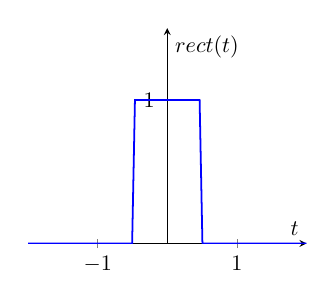
\begin{tikzpicture}[scale=0.8]
                \begin{axis}[
                    domain=-2:2,
                    samples=100,
                    axis lines=middle,
                    xlabel={$t$},
                    ylabel={$rect(t)$},
                    ymin=0, ymax=1.5,
                    xmin=-2, xmax=2,
                    xtick={-1,0,1},
                    ytick={0,1},
                    % grid=major,
                    height=5cm,
                    width=6cm
                ]
                    \addplot[thick,blue] {abs(x) <= 0.5 ? 1 : 0};
                \end{axis}
            \end{tikzpicture}
            \caption{Signal}
        \end{subfigure}
        \hfill
        % Sinc function
        \begin{subfigure}[b]{0.45\textwidth}
            \centering
            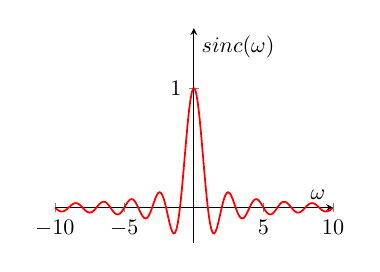
\begin{tikzpicture}[scale=0.8]
                \begin{axis}[
                    domain=-10:10,
                    samples=200,
                    axis lines=middle,
                    xlabel={$\omega$},
                    ylabel={$sinc(\omega)$},
                    ymin=-0.3, ymax=1.5,
                    xmin=-10, xmax=10,
                    xtick={-10,-5,5,10},
                    ytick={1},
                    % grid=major,
                    height=5cm,
                    width=6cm
                ]
                    \addplot[thick,red] {x == 0 ? 1 : sin(deg(pi*x))/(pi*x)};
                \end{axis}
            \end{tikzpicture}
            \caption{Fourier transformed signal}
        \end{subfigure}
    \end{figure}

\end{frame}

\begin{frame}
    \frametitle{Table of Content}
    \begin{itemize}[label=$\star$, itemsep=15pt, parsep=0pt, topsep=10pt]
        \item <1-> Fourier transform Formula
        \item <2-> Forward Fourier Transform
        \item <3-> Inverse Fourier Transform
        \item <4-> Fourier Transform Notation
        \item <5-> Properties of Fourier Transform
        \item <6-> Fourier Transform Table
    \end{itemize}
\end{frame}

\begin{frame}
    \frametitle{Fourier Transform Formula}
    There are \textcolor{red}{two types} of Fourier transform i.e., \textcolor{blue}{forward} Fourier transform and \textcolor{blue}{inverse} Fourier transform.\\
    The \textcolor{blue}{forward} Fourier transform of a continuous-time signal $x(t)$ is given by
    \begin{equation*}
        X(\omega) = \int_{-\infty}^{\infty} x(t) e^{-j\omega t} dt
    \end{equation*}
    The \textcolor{blue}{inverse} Fourier transform is given by
    \begin{equation*}
        x(t) = \int_{-\infty}^{\infty} X(\omega) e^{j\omega t} d\omega
    \end{equation*}
    where $\omega$ is the angular frequency, $j$ is the imaginary unit$(\sqrt{-1})$, and $t$ is the time.
\end{frame}

\begin{frame}
    \frametitle{Forward Fourier Transform}
    The forward Fourier transform is a mathematical technique used to transform a \textcolor{blue}{time-domain signal} into its \textcolor{blue}{frequency-domain} representation.
    The forward Fourier transform of a continuous-time signal $x(t)$ is given by
    \begin{equation*}
        X(\omega) = \int_{-\infty}^{\infty} x(t) e^{-j\omega t} dt
    \end{equation*}
    where $X(\omega)$ is the Fourier transform of $x(t)$.
\end{frame}

\begin{frame}
    \frametitle{Inverse Fourier Transform}
    The inverse Fourier transform is the process of \textcolor{blue}{converting a frequency-domain} representation of a signal \textcolor{blue}{back into its time-domain} form.
    The inverse Fourier transform is given by
    \begin{equation*}
        x(t) = \int_{-\infty}^{\infty} X(\omega) e^{j\omega t} d\omega
    \end{equation*}
    where $x(t)$ is the time-domain signal and $X(\omega)$ is the Fourier transform of $x(t)$.
\end{frame}

\begin{frame}
    \frametitle{Fourier Transform Notation}
    For convenience, we will write the Fourier transform of a signal $x(t)$ as
    \begin{equation*}
        X(f) = \mathcal{F}\{x(t)\}
    \end{equation*}
    and the inverse Fourier transform of $X(f)$ as
    \begin{equation*}
        x(t) = \mathcal{F}^{-1}\{X(f)\}
    \end{equation*}
    Note that
    \begin{equation*}
        \mathcal{F}^{-1}\{\mathcal{F}\{x(t)\}\} = x(t)
    \end{equation*}
    at points of continuity of x(t).
\end{frame}

\begin{frame}
    \frametitle{Example of Fourier Transform}
    Let $x(t) = rect(t)$ where rect(t) is the rectangular pulse function defined as
    \begin{equation*}
        rect(t) = \begin{cases}
            1 & \text{if } |t| < \frac{1}{2}\\
            0 & \text{otherwise}
        \end{cases}
    \end{equation*}
    and $sinc(\omega)$ is the sinc function defined as
    \begin{equation*}
        sinc(\omega) = \begin{cases}
            \frac{sin(\omega / 2)}{\omega / 2} & \text{if } \omega \neq 0\\
            1 & \text{if } \omega = 0
        \end{cases}
    \end{equation*}
    The forward Fourier transform of $rect(t)$ is $sinc(\omega)$ and the inverse Fourier transform of $sinc(\omega)$ is $rect(t)$.
\end{frame}

\begin{frame}
    \frametitle{Example of Fourier Transform}
    \begin{figure}[ht]
        \centering
        % Rect function
        \begin{subfigure}[b]{0.45\textwidth}
            \centering
            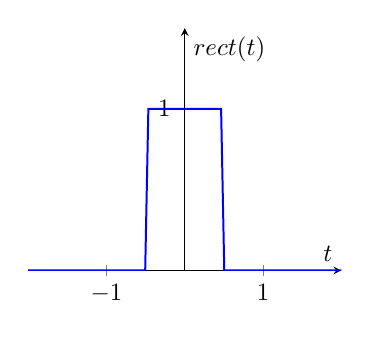
\begin{tikzpicture}[scale=0.9]
                \begin{axis}[
                    domain=-2:2,
                    samples=100,
                    axis lines=middle,
                    xlabel={$t$},
                    ylabel={$rect(t)$},
                    ymin=0, ymax=1.5,
                    xmin=-2, xmax=2,
                    xtick={-1,0,1},
                    ytick={0,1},
                    % grid=major,
                    height=5cm,
                    width=6cm
                ]
                    \addplot[thick,blue] {abs(x) <= 0.5 ? 1 : 0};
                \end{axis}
            \end{tikzpicture}
            \caption{Signal}
        \end{subfigure}
        \hfill
        % Sinc function
        \begin{subfigure}[b]{0.45\textwidth}
            \centering
            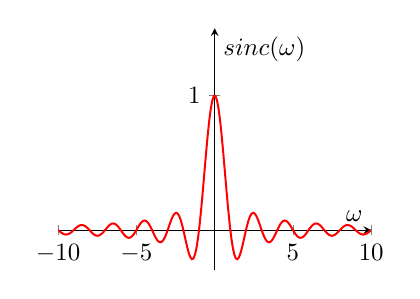
\begin{tikzpicture}[scale=0.9]
                \begin{axis}[
                    domain=-10:10,
                    samples=200,
                    axis lines=middle,
                    xlabel={$\omega$},
                    ylabel={$sinc(\omega)$},
                    ymin=-0.3, ymax=1.5,
                    xmin=-10, xmax=10,
                    xtick={-10,-5,5,10},
                    ytick={1},
                    % grid=major,
                    height=5cm,
                    width=6cm
                ]
                    \addplot[thick,red] {x == 0 ? 1 : sin(deg(pi*x))/(pi*x)};
                \end{axis}
            \end{tikzpicture}
            \caption{Fourier transformed signal}
        \end{subfigure}
    \end{figure}
\end{frame}

\begin{frame}
    \frametitle{Properties of Fourier Transform}
    \begin{itemize}[label=$\star$, itemsep=10pt, parsep=0pt, topsep=8pt]
        \item Linearity
        \item Time Shifting
        \item Frequency Shifting
        \item Time Scaling
        \item Time Reversal
        \item Differentiation
        \item Integration
        \item Convolution
    \end{itemize}
\end{frame}

\begin{frame}
    \frametitle{Properties of Fourier Transform}
    \setbeamercovered{dynamic, transparent = 20} % Enable dimming for unrevealed items

    % The list is shown in overlays where no details are displayed
    \only<1, 8, 12, 16, 20, 24, 28, 32>{
        \begin{itemize}[label=$\star$, itemsep=10pt, parsep=0pt, topsep=8pt]
            \item <1> Linearity
            \item <8> Time Shifting
            \item <12> Frequency Shifting
            \item <16> Time Scaling
            \item <20> Time Reversal
            \item <24> Differentiation
            \item <28> Integration
            \item <32> Convolution
        \end{itemize}
    }

    % Detailed content for Linearity
    \only<2>{
        \begin{block}{Linearity}
            The Fourier transform of a linear combination of signals is linear:
            \[
            F\{a x_1(t) + b x_2(t)\} = a X_1(\omega) + b X_2(\omega)
            \]
        \end{block}
    }

    \only<3>{
        \begin{block}{Linearity}
            Let $x_1(t) = rect(t - 1)$ and $x_2(t) = rect(t + 1)$ be two signals and let $X_1(\omega) = \mathcal{F} \{rect(t - 1)\}$ and $X_2(\omega) = \mathcal{F} \{rect(t + 1)\}$ be their fourier transforms respectively.
            \begin{figure}[ht]
                \centering
                % Rect(t - 1) and Fourier Transform
                \begin{subfigure}[b]{0.45\textwidth}
                    \centering
                    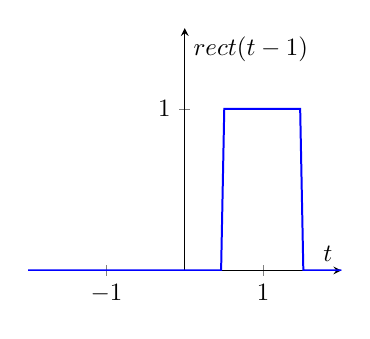
\begin{tikzpicture}[scale=0.9]
                        \begin{axis}[
                            domain=-2:2,
                            samples=100,
                            axis lines=middle,
                            xlabel={$t$},
                            ylabel={$rect(t - 1)$},
                            ymin=0, ymax=1.5,
                            xmin=-2, xmax=2,
                            xtick={-1,0,1},
                            ytick={0,1},
                            height=5cm,
                            width=6cm
                        ]
                            \addplot[thick,blue] {abs(x - 1) <= 0.5 ? 1 : 0};
                        \end{axis}
                    \end{tikzpicture}
                    \caption{$rect(t - 1)$}
                \end{subfigure}
                \hfill
                % Fourier Transform of rect(t - 1)
                \begin{subfigure}[b]{0.45\textwidth}
                    \centering
                    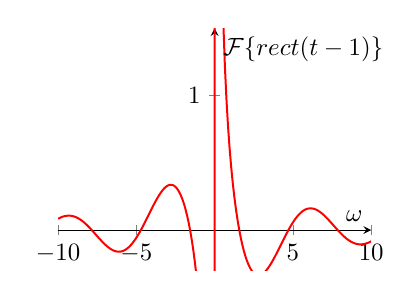
\begin{tikzpicture}[scale=0.9]
                        \begin{axis}[
                            domain=-10:10,
                            samples=200,
                            axis lines=middle,
                            xlabel={$\omega$},
                            ylabel={$\mathcal{F} \{rect(t - 1)\}$},
                            ymin=-0.3, ymax=1.5,
                            xmin=-10, xmax=10,
                            xtick={-10,-5,5,10},
                            ytick={1},
                            height=5cm,
                            width=6cm
                        ]
                            \addplot[thick,red] {cos(deg(x))/x};
                        \end{axis}
                    \end{tikzpicture}
                    \caption{$\mathcal{F} \{rect(t - 1)\}$}
                \end{subfigure}
            \end{figure}
        \end{block}
    }

    \only<4>{
        \begin{block}{Linearity}
            \begin{figure}[ht]
                \centering
                % 2 * rect(t - 1) and Fourier Transform
                \begin{subfigure}[b]{0.45\textwidth}
                    \centering
                    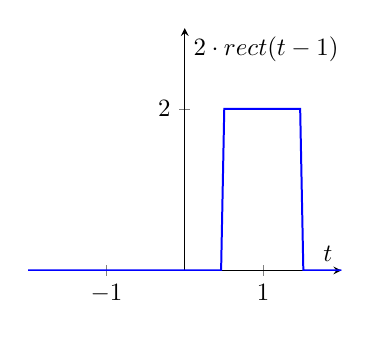
\begin{tikzpicture}[scale=0.9]
                        \begin{axis}[
                            domain=-2:2,
                            samples=100,
                            axis lines=middle,
                            xlabel={$t$},
                            ylabel={$2 \cdot rect(t - 1)$},
                            ymin=0, ymax=3,
                            xmin=-2, xmax=2,
                            xtick={-1,0,1},
                            ytick={0,2},
                            height=5cm,
                            width=6cm
                        ]
                            \addplot[thick,blue] {2 * (abs(x - 1) <= 0.5 ? 1 : 0)};
                        \end{axis}
                    \end{tikzpicture}
                    \caption{$2 \cdot rect(t - 1)$}
                \end{subfigure}
                \hfill
                % Fourier Transform of 2 * rect(t - 1)
                \begin{subfigure}[b]{0.45\textwidth}
                    \centering
                    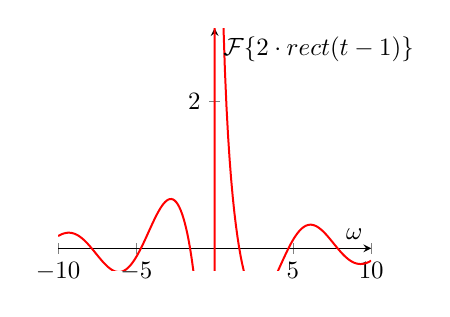
\begin{tikzpicture}[scale=0.9]
                        \begin{axis}[
                            domain=-10:10,
                            samples=200,
                            axis lines=middle,
                            xlabel={$\omega$},
                            ylabel={$\mathcal{F} \{2 \cdot rect(t - 1)\}$},
                            ymin=-0.3, ymax=3,
                            xmin=-10, xmax=10,
                            xtick={-10,-5,5,10},
                            ytick={2},
                            height=5cm,
                            width=6cm
                        ]
                            \addplot[thick,red] {2 * cos(deg(x))/x};
                        \end{axis}
                    \end{tikzpicture}
                    \caption{$\mathcal{F} \{2 \cdot rect(t - 1)\}$}
                \end{subfigure}
            \end{figure}
            Here,
            \begin{equation*}
                \mathcal{F} \{2 \cdot rect(t - 1)\} = 2 \cdot \mathcal{F} \{rect(t - 1)\}
            \end{equation*}
        \end{block}
    }

    \only<5>{
        \begin{block}{Linearity}
            \begin{figure}[ht]
                \centering
                % rect(t + 1) and Fourier Transform
                \begin{subfigure}[b]{0.45\textwidth}
                    \centering
                    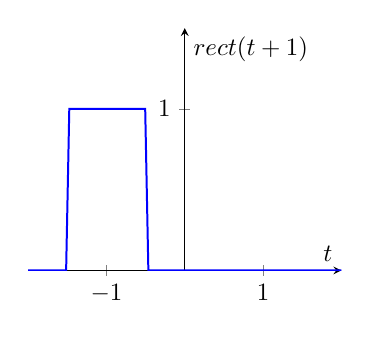
\begin{tikzpicture}[scale=0.9]
                        \begin{axis}[
                            domain=-2:2,
                            samples=100,
                            axis lines=middle,
                            xlabel={$t$},
                            ylabel={$rect(t + 1)$},
                            ymin=0, ymax=1.5,
                            xmin=-2, xmax=2,
                            xtick={-1,0,1},
                            ytick={0,1},
                            height=5cm,
                            width=6cm
                        ]
                            \addplot[thick,blue] {abs(x + 1) <= 0.5 ? 1 : 0};
                        \end{axis}
                    \end{tikzpicture}
                    \caption{$rect(t + 1)$}
                \end{subfigure}
                \hfill
                % Fourier Transform of rect(t + 1)
                \begin{subfigure}[b]{0.45\textwidth}
                    \centering
                    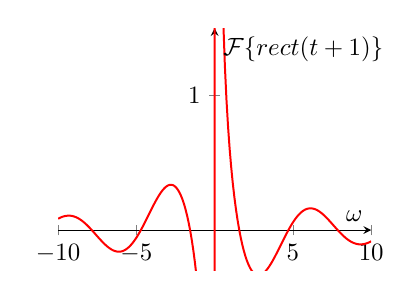
\begin{tikzpicture}[scale=0.9]
                        \begin{axis}[
                            domain=-10:10,
                            samples=200,
                            axis lines=middle,
                            xlabel={$\omega$},
                            ylabel={$\mathcal{F} \{rect(t + 1)\}$},
                            ymin=-0.3, ymax=1.5,
                            xmin=-10, xmax=10,
                            xtick={-10,-5,5,10},
                            ytick={1},
                            height=5cm,
                            width=6cm
                        ]
                            \addplot[thick,red] {cos(deg(x))/x};
                        \end{axis}
                    \end{tikzpicture}
                    \caption{$\mathcal{F} \{rect(t + 1)\}$}
                \end{subfigure}
            \end{figure}
        \end{block}
    }

    \only<6>{
        \begin{block}{Linearity}
            \begin{figure}
                \centering
                % 3 * rect(t + 1) and Fourier Transform
                \begin{subfigure}[b]{0.45\textwidth}
                    \centering
                    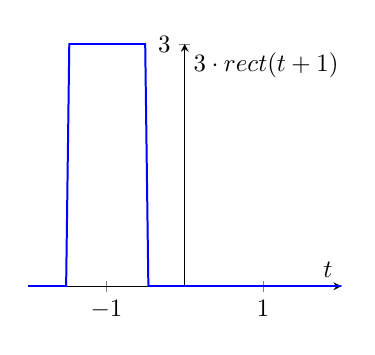
\begin{tikzpicture}[scale=0.9]
                        \begin{axis}[
                            domain=-2:2,
                            samples=100,
                            axis lines=middle,
                            xlabel={$t$},
                            ylabel={$3 \cdot rect(t + 1)$},
                            ymin=0, ymax=3,
                            xmin=-2, xmax=2,
                            xtick={-1,0,1},
                            ytick={0,3},
                            height=5cm,
                            width=6cm
                        ]
                            \addplot[thick,blue] {3 * (abs(x + 1) <= 0.5 ? 1 : 0)};
                        \end{axis}
                    \end{tikzpicture}
                    \caption{$3 \cdot rect(t + 1)$}
                \end{subfigure}
                \hfill
                % Fourier Transform of 3 * rect(t + 1)
                \begin{subfigure}[b]{0.45\textwidth}
                    \centering
                    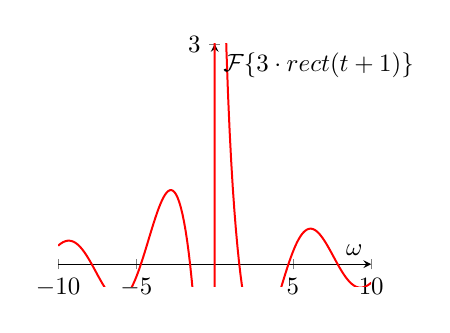
\begin{tikzpicture}[scale=0.9]
                        \begin{axis}[
                            domain=-10:10,
                            samples=200,
                            axis lines=middle,
                            xlabel={$\omega$},
                            ylabel={$\mathcal{F} \{3 \cdot rect(t + 1)\}$},
                            ymin=-0.3, ymax=3,
                            xmin=-10, xmax=10,
                            xtick={-10,-5,5,10},
                            ytick={3},
                            height=5cm,
                            width=6cm
                        ]
                            \addplot[thick,red] {3 * cos(deg(x))/x};
                        \end{axis}
                    \end{tikzpicture}
                    \caption{$\mathcal{F} \{3 \cdot rect(t + 1)\}$}
                \end{subfigure}
            \end{figure}
            Here,
            \begin{equation*}
                \mathcal{F} \{3 \cdot rect(t + 1)\} = 3 \cdot \mathcal{F} \{rect(t + 1)\}
            \end{equation*}
        \end{block}
    }

    \only<7>{
        \begin{block}{Linearity}
            \begin{figure}
                \centering
                % 2 * rect(t - 1) + 3 * rect(t + 1) and Fourier Transform
                \begin{subfigure}[b]{0.45\textwidth}
                    \centering
                    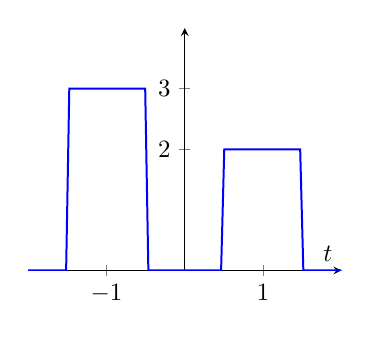
\begin{tikzpicture}[scale=0.9]
                        \begin{axis}[
                            domain=-2:2,
                            samples=100,
                            axis lines=middle,
                            xlabel={$t$},
                            % ylabel={$2 \cdot rect(t - 1) + 3 \cdot rect(t + 1)$},
                            ymin=0, ymax=4,
                            xmin=-2, xmax=2,
                            xtick={-1,0,1},
                            ytick={2,3},
                            height=5cm,
                            width=6cm
                        ]
                            \addplot[thick,blue] {2 * (abs(x - 1) <= 0.5 ? 1 : 0) + 3 * (abs(x + 1) <= 0.5 ? 1 : 0)};
                        \end{axis}
                    \end{tikzpicture}
                    \caption{$2 \cdot rect(t - 1) + 3 \cdot rect(t + 1)$}
                \end{subfigure}
                \hfill
                % Fourier Transform of 2 * rect(t - 1) + 3 * rect(t + 1)
                \begin{subfigure}[b]{0.45\textwidth}
                    \centering
                    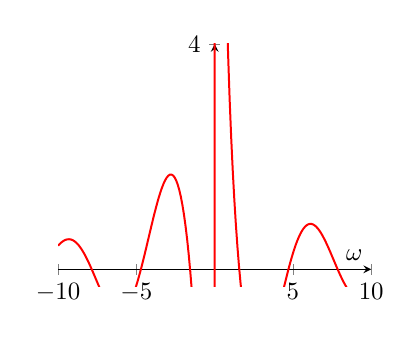
\begin{tikzpicture}[scale=0.9]
                        \begin{axis}[
                            domain=-10:10,
                            samples=200,
                            axis lines=middle,
                            xlabel={$\omega$},
                            % ylabel={$\mathcal{F} \{2 \cdot rect(t - 1) + 3 \cdot rect(t + 1)\}$},
                            ymin=-0.3, ymax=4,
                            xmin=-10, xmax=10,
                            xtick={-10,-5,5,10},
                            ytick={4},
                            height=5cm,
                            width=6cm
                        ]
                            \addplot[thick,red] {2 * cos(deg(x))/x + 3 * cos(deg(x))/x};
                        \end{axis}
                    \end{tikzpicture}
                    \caption{$\mathcal{F} \{2 \cdot rect(t - 1) + 3 \cdot rect(t + 1)\}$}
                \end{subfigure}
            \end{figure}
            Here,
            \begin{equation*}
                \mathcal{F} \{2 \cdot rect(t - 1) + 3 \cdot rect(t + 1)\} = 2 \cdot \mathcal{F} \{rect(t - 1)\} + 3 \cdot \mathcal{F} \{rect(t + 1)\}
            \end{equation*}
        \end{block}
    }

    % Detailed content for Time Shifting
    \only<9>{
        \begin{block}{Time Shifting}
            Shifting a signal in time corresponds to a phase shift in its Fourier transform:
            \[
            x(t - t_0) \xrightarrow{\text{FT}} X(\omega)e^{-j\omega t_0}
            \]
        \end{block}
    }

    \only<10>{
        \begin{block}{Time Shifting}
            Let $x(t) = rect(t)$ be a signal with Fourier transform $X(\omega) = \mathcal{F} \{rect(t)\}$.
            \begin{figure}[ht]
                \centering
                % rect(t) and Fourier Transform
                \begin{subfigure}[b]{0.45\textwidth}
                    \centering
                    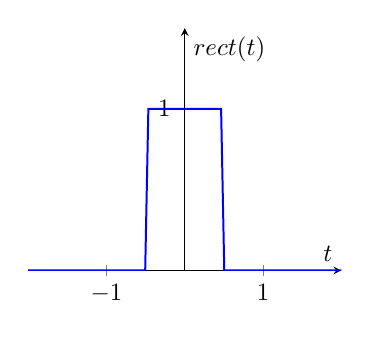
\begin{tikzpicture}[scale=0.9]
                        \begin{axis}[
                            domain=-2:2,
                            samples=100,
                            axis lines=middle,
                            xlabel={$t$},
                            ylabel={$rect(t)$},
                            ymin=0, ymax=1.5,
                            xmin=-2, xmax=2,
                            xtick={-1,0,1},
                            ytick={0,1},
                            height=5cm,
                            width=6cm
                        ]
                            \addplot[thick,blue] {abs(x) <= 0.5 ? 1 : 0};
                        \end{axis}
                    \end{tikzpicture}
                    \caption{$rect(t)$}
                \end{subfigure}
                \hfill
                % Fourier Transform of rect(t)
                \begin{subfigure}[b]{0.45\textwidth}
                    \centering
                    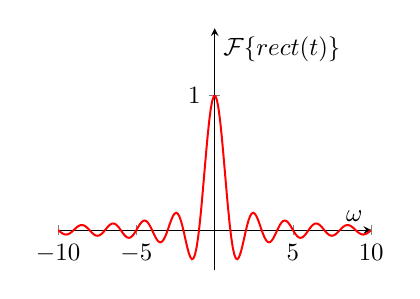
\begin{tikzpicture}[scale=0.9]
                        \begin{axis}[
                            domain=-10:10,
                            samples=200,
                            axis lines=middle,
                            xlabel={$\omega$},
                            ylabel={$\mathcal{F} \{rect(t)\}$},
                            ymin=-0.3, ymax=1.5,
                            xmin=-10, xmax=10,
                            xtick={-10,-5,5,10},
                            ytick={1},
                            % grid=major,
                            height=5cm,
                            width=6cm
                        ]
                            \addplot[thick,red] {x == 0 ? 1 : sin(deg(pi*x))/(pi*x)};
                        \end{axis}
                    \end{tikzpicture}
                    \caption{$\mathcal{F} \{rect(t)\}$}
                \end{subfigure}
            \end{figure}
        \end{block}
    }

    \only<11>{
        \begin{block}{Time Shifting}
            \begin{figure}
                \centering
                % rect(t - 1) and Fourier Transform
                \begin{subfigure}[b]{0.45\textwidth}
                    \centering
                    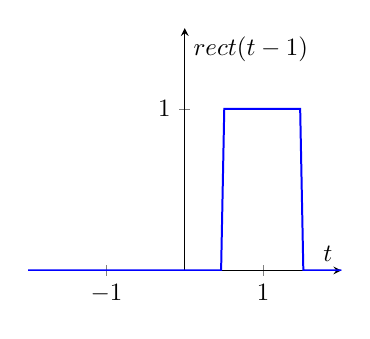
\begin{tikzpicture}[scale=0.9]
                        \begin{axis}[
                            domain=-2:2,
                            samples=100,
                            axis lines=middle,
                            xlabel={$t$},
                            ylabel={$rect(t - 1)$},
                            ymin=0, ymax=1.5,
                            xmin=-2, xmax=2,
                            xtick={-1,0,1},
                            ytick={0,1},
                            height=5cm,
                            width=6cm
                        ]
                            \addplot[thick,blue] {abs(x - 1) <= 0.5 ? 1 : 0};
                        \end{axis}
                    \end{tikzpicture}
                    \caption{$rect(t - 1)$}
                \end{subfigure}
                \hfill
                % Fourier Transform of rect(t - 1)
                \begin{subfigure}[b]{0.45\textwidth}
                    \centering
                    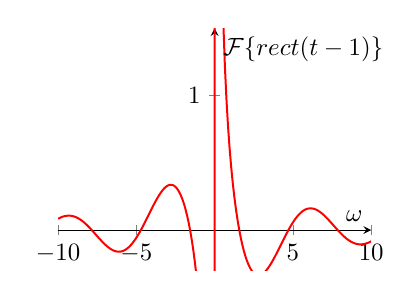
\begin{tikzpicture}[scale=0.9]
                        \begin{axis}[
                            domain=-10:10,
                            samples=200,
                            axis lines=middle,
                            xlabel={$\omega$},
                            ylabel={$\mathcal{F} \{rect(t - 1)\}$},
                            ymin=-0.3, ymax=1.5,
                            xmin=-10, xmax=10,
                            xtick={-10,-5,5,10},
                            ytick={1},
                            height=5cm,
                            width=6cm
                        ]
                            \addplot[thick,red] {cos(deg(x))/x};
                        \end{axis}
                    \end{tikzpicture}
                    \caption{$\mathcal{F} \{rect(t - 1)\}$}
                \end{subfigure}
            \end{figure}
        \end{block}
    }

    % Detailed content for Frequency Shifting
    \only<13>{
        \begin{block}{Frequency Shifting}
            Shifting in frequency results in modulation of the time-domain signal:
            \[
            X(\omega - \omega_0) \xrightarrow{\text{IFT}} x(t)e^{j\omega_0 t}
            \]
        \end{block}
    }

    \only<14>{
        \begin{block}{Frequency Shifting}
            Let $X(\omega) = \frac{sin\frac{\omega}{2}}{\frac{\omega}{2}}$ and $x(t) = \mathcal{F}^{-1}\{X(\omega)\}$ is the inverse Fourier transform of $X(\omega)$.
            \begin{figure}
                \centering
                % Sinc function
                \begin{subfigure}[b]{0.45\textwidth}
                    \centering
                    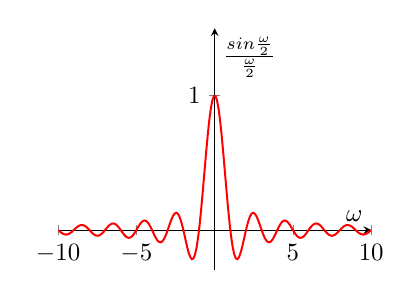
\begin{tikzpicture}[scale=0.9]
                        \begin{axis}[
                            domain=-10:10,
                            samples=200,
                            axis lines=middle,
                            xlabel={$\omega$},
                            ylabel={$\frac{sin\frac{\omega}{2}}{\frac{\omega}{2}}$},
                            ymin=-0.3, ymax=1.5,
                            xmin=-10, xmax=10,
                            xtick={-10,-5,5,10},
                            ytick={1},
                            height=5cm,
                            width=6cm
                        ]
                            \addplot[thick,red] {x == 0 ? 1 : sin(deg(pi*x))/(pi*x)};
                        \end{axis}
                    \end{tikzpicture}
                    \caption{$\frac{sin\frac{\omega}{2}}{\frac{\omega}{2}}$}
                \end{subfigure}
                \hfill
                % Inverse Fourier Transform of sinc function
                \begin{subfigure}[b]{0.45\textwidth}
                    \centering
                    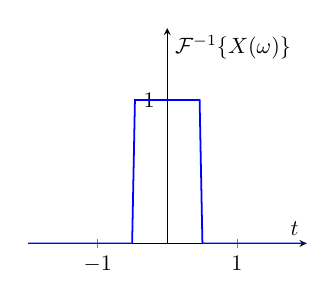
\begin{tikzpicture}[scale=0.8]
                        \begin{axis}[
                            domain=-2:2,
                            samples=100,
                            axis lines=middle,
                            xlabel={$t$},
                            ylabel={$\mathcal{F}^{-1}\{X(\omega)\}$},
                            ymin=0, ymax=1.5,
                            xmin=-2, xmax=2,
                            xtick={-1,0,1},
                            ytick={0,1},
                            % grid=major,
                            height=5cm,
                            width=6cm
                        ]
                            \addplot[thick,blue] {abs(x) <= 0.5 ? 1 : 0};
                        \end{axis}
                    \end{tikzpicture}
                    \caption{$\mathcal{F}^{-1}\{X(\omega)\}$}
                \end{subfigure}
            \end{figure}
        \end{block}
    }

    \only<15>{
        \begin{block}{Frequency Shifting}
            \begin{figure}
                \centering
                % Frequency shifted signal
                \begin{subfigure}[b]{0.45\textwidth}
                    \centering
                    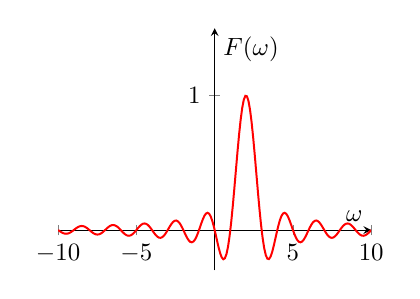
\begin{tikzpicture}[scale=0.9]
                        \begin{axis}[
                            domain=-10:10,
                            samples=200,
                            axis lines=middle,
                            xlabel={$\omega$},
                            ylabel={$F(\omega)$},
                            ymin=-0.3, ymax=1.5,
                            xmin=-10, xmax=10,
                            xtick={-10,-5,5,10},
                            ytick={1},
                            height=5cm,
                            width=6cm
                        ]
                            \addplot[thick,red] {x == 2 ? 1 : sin(deg(pi*(x - 2)))/(pi*(x - 2))};
                        \end{axis}
                    \end{tikzpicture}
                    \caption{$\frac{\sin\left(\frac{\omega - 2}{2}\right)}{\frac{\omega - 2}{2}}$}
                \end{subfigure}
                \hfill
                % Inverse Fourier Transform of frequency shifted signal
                \begin{subfigure}[b]{0.45\textwidth}
                    \centering
                    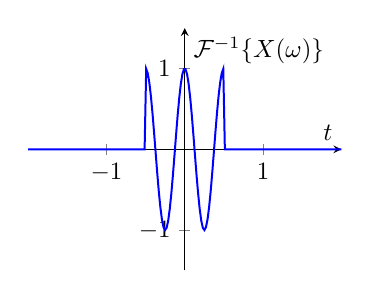
\begin{tikzpicture}[scale=0.9]
                        \begin{axis}[
                            domain=-2:2,
                            samples=200,
                            axis lines=middle,
                            xlabel={$t$},
                            ylabel={$\mathcal{F}^{-1}\{X(\omega)\}$},
                            ymin=-1.5, ymax=1.5,
                            xmin=-2, xmax=2,
                            xtick={-1,0,1},
                            ytick={-1,0,1},
                            height=5cm,
                            width=6cm
                        ]
                            \addplot[thick,blue] {(abs(x) <= 0.5) * cos(deg(2*pi*2*x))};
                        \end{axis}
                    \end{tikzpicture}
                    \caption{$\mathcal{F}^{-1}\{X(\omega)\}$}
                \end{subfigure}
            \end{figure}
        \end{block}
    }

    % Detailed content for Time Scaling
    \only<17>{
        \begin{block}{Time Scaling}
            Stretching or compressing a signal in time inversely scales its frequency spectrum:
            \[
            x(at) \xrightarrow{\text{FT}} \frac{1}{|a|}X\left(\frac{\omega}{a}\right)
            \]
        \end{block}
    }

    \only<18>{
        \begin{block}{Time Scaling}
            Let $x(t) = rect(t)$ be a signal with Fourier transform $X(\omega) = \mathcal{F} \{rect(t)\}$.
            \begin{figure}
                \centering
                % Rect function
                \begin{subfigure}[b]{0.45\textwidth}
                    \centering
                    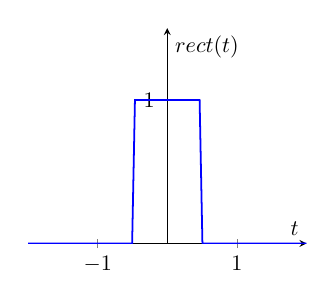
\begin{tikzpicture}[scale=0.8]
                        \begin{axis}[
                            domain=-2:2,
                            samples=100,
                            axis lines=middle,
                            xlabel={$t$},
                            ylabel={$rect(t)$},
                            ymin=0, ymax=1.5,
                            xmin=-2, xmax=2,
                            xtick={-1,0,1},
                            ytick={0,1},
                            % grid=major,
                            height=5cm,
                            width=6cm
                        ]
                            \addplot[thick,blue] {abs(x) <= 0.5 ? 1 : 0};
                        \end{axis}
                    \end{tikzpicture}
                    \caption{Signal}
                \end{subfigure}
                \hfill
                % Sinc function
                \begin{subfigure}[b]{0.45\textwidth}
                    \centering
                    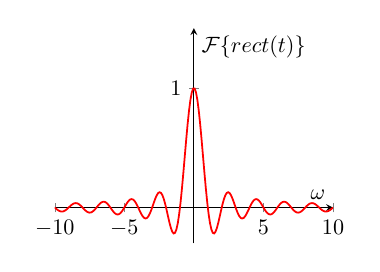
\begin{tikzpicture}[scale=0.8]
                        \begin{axis}[
                            domain=-10:10,
                            samples=200,
                            axis lines=middle,
                            xlabel={$\omega$},
                            ylabel={$\mathcal{F} \{rect(t)\}$},
                            ymin=-0.3, ymax=1.5,
                            xmin=-10, xmax=10,
                            xtick={-10,-5,5,10},
                            ytick={1},
                            % grid=major,
                            height=5cm,
                            width=6cm
                        ]
                            \addplot[thick,red] {x == 0 ? 1 : sin(deg(pi*x))/(pi*x)};
                        \end{axis}
                    \end{tikzpicture}
                    \caption{$\mathcal{F} \{rect(t)\}$}
                \end{subfigure}
            \end{figure}
        \end{block}
    }

    \only<19>{
        \begin{block}{Time Scaling}
            \begin{figure}
                \centering
                % Time domain signal rect(2t)
                \begin{subfigure}[b]{0.45\textwidth}
                    \centering
                    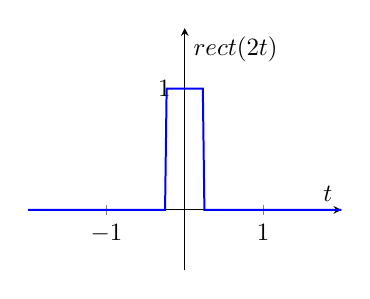
\begin{tikzpicture}[scale=0.9]
                        \begin{axis}[
                            domain=-2:2,
                            samples=200,
                            axis lines=middle,
                            xlabel={$t$},
                            ylabel={$rect(2t)$},
                            ymin=-0.5, ymax=1.5,
                            xmin=-2, xmax=2,
                            xtick={-1,0,1},
                            ytick={0,1},
                            height=5cm,
                            width=6cm
                        ]
                            \addplot[thick,blue] {abs(2*x) <= 0.5 ? 1 : 0};
                        \end{axis}
                    \end{tikzpicture}
                    \caption{$rect(2t)$}
                \end{subfigure}
                \hfill
                % Fourier Transform of rect(2t)
                \begin{subfigure}[b]{0.45\textwidth}
                    \centering
                    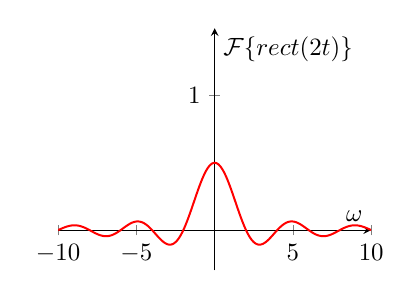
\begin{tikzpicture}[scale=0.9]
                        \begin{axis}[
                            domain=-10:10,
                            samples=200,
                            axis lines=middle,
                            xlabel={$\omega$},
                            ylabel={$\mathcal{F} \{rect(2t)\}$},
                            ymin=-0.3, ymax=1.5,
                            xmin=-10, xmax=10,
                            xtick={-10,-5,0,5,10},
                            ytick={1},
                            height=5cm,
                            width=6cm
                        ]
                            \addplot[thick,red] {(sin(deg(pi*x/2))/(pi*x/2))/2};
                        \end{axis}
                    \end{tikzpicture}
                    \caption{$\mathcal{F} \{rect(2t)\}$}
                \end{subfigure}
            \end{figure}
        \end{block}
    }

    % Detailed content for Time Reversal
    \only<21>{
        \begin{block}{Time Reversal}
            \textcolor{red}{Time reversal} in the time domain corresponds to \textcolor{red}{frequency reversal} in the frequency domain:
            \[
            x(-t) \xrightarrow{\text{FT}} X(-\omega)
            \]
        \end{block}
    }

    \only<22>{
        \begin{block}{Time Reversal}
            Let $x(t) = rect(t)$ be a signal with Fourier transform $X(\omega) = \mathcal{F} \{rect(t)\}$.
            \begin{figure}
                \centering
                % Rect function
                \begin{subfigure}[b]{0.45\textwidth}
                    \centering
                    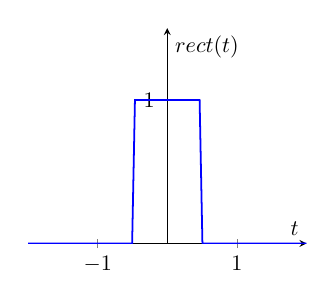
\begin{tikzpicture}[scale=0.8]
                        \begin{axis}[
                            domain=-2:2,
                            samples=100,
                            axis lines=middle,
                            xlabel={$t$},
                            ylabel={$rect(t)$},
                            ymin=0, ymax=1.5,
                            xmin=-2, xmax=2,
                            xtick={-1,0,1},
                            ytick={0,1},
                            % grid=major,
                            height=5cm,
                            width=6cm
                        ]
                            \addplot[thick,blue] {abs(x) <= 0.5 ? 1 : 0};
                        \end{axis}
                    \end{tikzpicture}
                    \caption{Signal}
                \end{subfigure}
                \hfill
                % Sinc function
                \begin{subfigure}[b]{0.45\textwidth}
                    \centering
                    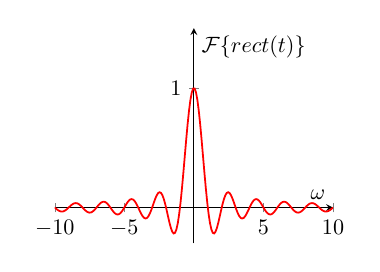
\begin{tikzpicture}[scale=0.8]
                        \begin{axis}[
                            domain=-10:10,
                            samples=200,
                            axis lines=middle,
                            xlabel={$\omega$},
                            ylabel={$\mathcal{F} \{rect(t)\}$},
                            ymin=-0.3, ymax=1.5,
                            xmin=-10, xmax=10,
                            xtick={-10,-5,5,10},
                            ytick={1},
                            % grid=major,
                            height=5cm,
                            width=6cm
                        ]
                            \addplot[thick,red] {x == 0 ? 1 : sin(deg(pi*x))/(pi*x)};
                        \end{axis}
                    \end{tikzpicture}
                    \caption{$\mathcal{F} \{rect(t)\}$}
                \end{subfigure}
            \end{figure}
        \end{block}
    }

    \only<23>{
        \begin{block}{Time Reversal}
            \begin{figure}[ht]
                \centering
                % Time domain signal rect(-t)
                \begin{subfigure}[b]{0.45\textwidth}
                    \centering
                    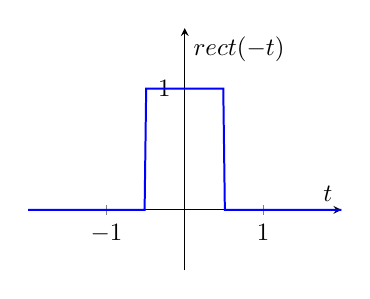
\begin{tikzpicture}[scale=0.9]
                        \begin{axis}[
                            domain=-2:2,
                            samples=200,
                            axis lines=middle,
                            xlabel={$t$},
                            ylabel={$rect(-t)$},
                            ymin=-0.5, ymax=1.5,
                            xmin=-2, xmax=2,
                            xtick={-1,0,1},
                            ytick={0,1},
                            height=5cm,
                            width=6cm
                        ]
                            \addplot[thick,blue] {abs(-x) <= 0.5 ? 1 : 0};
                        \end{axis}
                    \end{tikzpicture}
                    \caption{$rect(-t)$}
                \end{subfigure}
                \hfill
                % Fourier Transform of rect(-t)
                \begin{subfigure}[b]{0.45\textwidth}
                    \centering
                    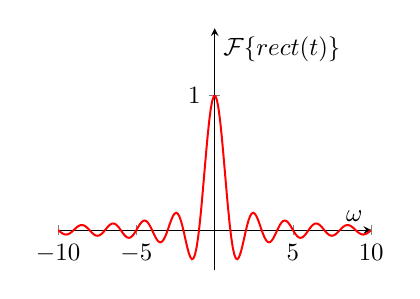
\begin{tikzpicture}[scale=0.9]
                        \begin{axis}[
                            domain=-10:10,
                            samples=200,
                            axis lines=middle,
                            xlabel={$\omega$},
                            ylabel={$\mathcal{F} \{rect(t)\}$},
                            ymin=-0.3, ymax=1.5,
                            xmin=-10, xmax=10,
                            xtick={-10,-5,0,5,10},
                            ytick={1},
                            height=5cm,
                            width=6cm
                        ]
                            \addplot[thick,red] {(sin(deg(pi*x))/(pi*x))};
                        \end{axis}
                    \end{tikzpicture}
                    \caption{$\mathcal{F} \{rect(t)\}$}
                \end{subfigure}
            \end{figure}
        \end{block}
    }

    % Detailed content for Time Differentiation
    \only<25>{
        \begin{block}{Differentiation}
            Differentiation in the time domain corresponds to multiplication by $j\omega$ in the frequency domain:
            \[
            \frac{d}{dt}x(t) \xrightarrow{\text{FT}} j\omega X(\omega)
            \]
        \end{block}
    }

    \only<26>{
        \begin{block}{Differentiation}
            Let $x(t) = rect(t)$ be a signal with Fourier transform $X(\omega) = \mathcal{F} \{rect(t)\}$.
            \begin{figure}
                \centering
                % Rect function
                \begin{subfigure}[b]{0.45\textwidth}
                    \centering
                    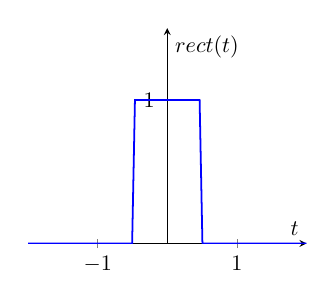
\begin{tikzpicture}[scale=0.8]
                        \begin{axis}[
                            domain=-2:2,
                            samples=100,
                            axis lines=middle,
                            xlabel={$t$},
                            ylabel={$rect(t)$},
                            ymin=0, ymax=1.5,
                            xmin=-2, xmax=2,
                            xtick={-1,0,1},
                            ytick={0,1},
                            % grid=major,
                            height=5cm,
                            width=6cm
                        ]
                            \addplot[thick,blue] {abs(x) <= 0.5 ? 1 : 0};
                        \end{axis}
                    \end{tikzpicture}
                    \caption{Signal}
                \end{subfigure}
                \hfill
                % Sinc function
                \begin{subfigure}[b]{0.45\textwidth}
                    \centering
                    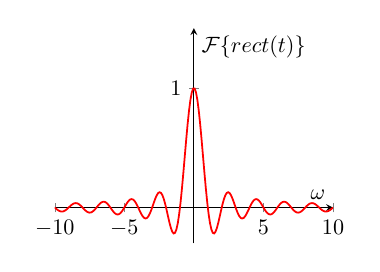
\begin{tikzpicture}[scale=0.8]
                        \begin{axis}[
                            domain=-10:10,
                            samples=200,
                            axis lines=middle,
                            xlabel={$\omega$},
                            ylabel={$\mathcal{F} \{rect(t)\}$},
                            ymin=-0.3, ymax=1.5,
                            xmin=-10, xmax=10,
                            xtick={-10,-5,5,10},
                            ytick={1},
                            % grid=major,
                            height=5cm,
                            width=6cm
                        ]
                            \addplot[thick,red] {x == 0 ? 1 : sin(deg(pi*x))/(pi*x)};
                        \end{axis}
                    \end{tikzpicture}
                    \caption{$\mathcal{F} \{rect(t)\}$}
                \end{subfigure}
            \end{figure}
        \end{block}
    }

    \only<27>{
        \begin{block}{Differentiation}
            \begin{figure}
                \centering
                % Differentiated signal
                \begin{subfigure}[b]{0.45\textwidth}
                    \centering
                    \begin{tikzpicture}[scale=0.9]
                        \begin{axis}[
                            domain=-2:2,
                            samples=200,
                            axis lines=middle,
                            xlabel={$t$},
                            ylabel={$\frac{d}{dt}rect(t)$},
                            ymin=-1.5, ymax=1.5,
                            xmin=-2, xmax=2,
                            xtick={-1,0,1},
                            ytick={-1,0,1},
                            height=5cm,
                            width=6cm
                        ]
                            \addplot[only marks,mark=triangle*,mark options={scale=2,fill=blue}] coordinates {(-0.5,-1)};
                            \addplot[only marks,mark=triangle*,mark options={scale=2,fill=red}] coordinates {(0.5,1)};
                        \end{axis}
                    \end{tikzpicture}
                    \caption{$\frac{d}{dt}rect(t)$}
                \end{subfigure}
                \hfill
                % Fourier Transform of differentiated signal
                \begin{subfigure}[b]{0.45\textwidth}
                    \centering
                    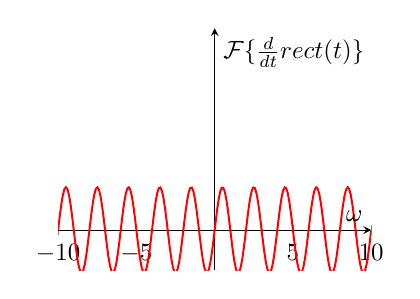
\begin{tikzpicture}[scale=0.9]
                        \begin{axis}[
                            domain=-10:10,
                            samples=200,
                            axis lines=middle,
                            xlabel={$\omega$},
                            ylabel={$\mathcal{F} \{\frac{d}{dt}rect(t)\}$},
                            ymin=-0.3, ymax=1.5,
                            xmin=-10, xmax=10,
                            xtick={-10,-5,0,5,10},
                            ytick={0},
                            height=5cm,
                            width=6cm
                        ]
                            \addplot[thick,red] {x*sin(deg(pi*x))/(pi*x)};
                        \end{axis}
                    \end{tikzpicture}
                    \caption{$\mathcal{F} \{\frac{d}{dt}rect(t)\}$}
                \end{subfigure}
            \end{figure}
        \end{block}
    }

    % Detailed content for Time Integration
    \only<29>{
        \begin{block}{Integration}
            Integration in the time domain corresponds to multiplication by $\frac{1}{j\omega}$ in the frequency domain:
            \[
            \int x(t)dt \xrightarrow{\text{FT}} \frac{1}{j\omega}X(\omega)
            \]
        \end{block}
    }

    \only<30>{
        \begin{block}{Integration}
            Let $x(t) = rect(t)$ be a signal with Fourier transform $X(\omega) = \mathcal{F} \{rect(t)\}$.
            \begin{figure}
                \centering
                % Rect function
                \begin{subfigure}[b]{0.45\textwidth}
                    \centering
                    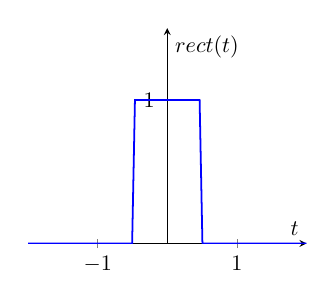
\begin{tikzpicture}[scale=0.8]
                        \begin{axis}[
                            domain=-2:2,
                            samples=100,
                            axis lines=middle,
                            xlabel={$t$},
                            ylabel={$rect(t)$},
                            ymin=0, ymax=1.5,
                            xmin=-2, xmax=2,
                            xtick={-1,0,1},
                            ytick={0,1},
                            % grid=major,
                            height=5cm,
                            width=6cm
                        ]
                            \addplot[thick,blue] {abs(x) <= 0.5 ? 1 : 0};
                        \end{axis}
                    \end{tikzpicture}
                    \caption{Signal}
                \end{subfigure}
                \hfill
                % Sinc function
                \begin{subfigure}[b]{0.45\textwidth}
                    \centering
                    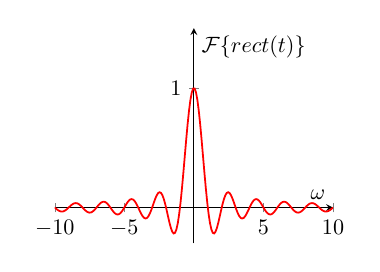
\begin{tikzpicture}[scale=0.8]
                        \begin{axis}[
                            domain=-10:10,
                            samples=200,
                            axis lines=middle,
                            xlabel={$\omega$},
                            ylabel={$\mathcal{F} \{rect(t)\}$},
                            ymin=-0.3, ymax=1.5,
                            xmin=-10, xmax=10,
                            xtick={-10,-5,5,10},
                            ytick={1},
                            % grid=major,
                            height=5cm,
                            width=6cm
                        ]
                            \addplot[thick,red] {x == 0 ? 1 : sin(deg(pi*x))/(pi*x)};
                        \end{axis}
                    \end{tikzpicture}
                    \caption{$\mathcal{F} \{rect(t)\}$}
                \end{subfigure}
            \end{figure}
        \end{block}
    }

    \only<31>{
        \begin{block}{Integration}
            \begin{figure}
                \centering
                % Integrated signal
                \begin{subfigure}[b]{0.45\textwidth}
                    \centering
                    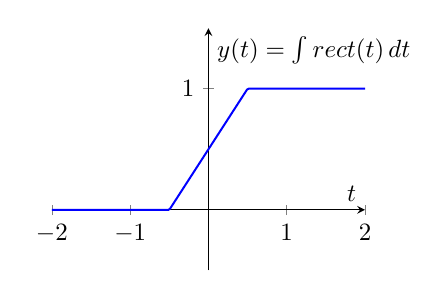
\begin{tikzpicture}[scale=0.9]
                        \begin{axis}[
                            domain=-2:2,
                            samples=200,
                            axis lines=middle,
                            xlabel={$t$},
                            ylabel={$y(t) = \int rect(t) \, dt$},
                            ymin=-0.5, ymax=1.5,
                            xmin=-2, xmax=2,
                            xtick={-2,-1,0,1,2},
                            ytick={0,1},
                            height=5cm,
                            width=6cm
                        ]
                            \addplot[thick,blue] {x <= -0.5 ? 0 : (x < 0.5 ? x + 0.5 : 1)};
                        \end{axis}
                    \end{tikzpicture}
                    \caption{$y(t) = \int rect(t) dt$}
                \end{subfigure}
                \hfill
                % Fourier Transform of integrated signal
                \begin{subfigure}[b]{0.45\textwidth}
                    \centering
                    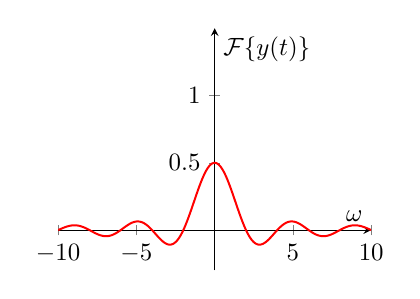
\begin{tikzpicture}[scale=0.9]
                        \begin{axis}[
                            domain=-10:10,
                            samples=200,
                            axis lines=middle,
                            xlabel={$\omega$},
                            ylabel={$\mathcal{F} \{y(t)\}$},
                            ymin=-0.3, ymax=1.5,
                            xmin=-10, xmax=10,
                            xtick={-10,-5,0,5,10},
                            ytick={0,0.5,1},
                            height=5cm,
                            width=6cm
                        ]
                            \addplot[thick,red] {x == 0 ? 0.5 : 1/(pi*x)*sin(deg(pi*x/2))};
                        \end{axis}
                    \end{tikzpicture}
                    \caption{$\mathcal{F} \{y(t)\}$}
                \end{subfigure}
            \end{figure}
        \end{block}
    }

    % Detailed content for Time Convolution
    \only<33>{
        \begin{block}{Convolution}
            Convolution in the time domain corresponds to multiplication in the frequency domain:
            \[
            x(t) * y(t) \xrightarrow{\text{FT}} X(\omega)Y(\omega)
            \]
        \end{block}
    }

    \only<34>{
        \begin{block}{Convolution}
            Let $x(t) = rect(t)$ and $y(t) = rect(t)$ be signals with Fourier transforms $X(\omega) = \mathcal{F} \{rect(t)\}$ and $Y(\omega) = \mathcal{F} \{rect(t)\}$. The convolution in the time domain corresponds to the product in the frequency domain:
            \[
            z(t) = x(t) * y(t) \quad \leftrightarrow \quad Z(\omega) = X(\omega) \cdot Y(\omega).
            \]
            \begin{figure}
                \centering
                % Rect function
                \begin{subfigure}[b]{0.45\textwidth}
                    \centering
                    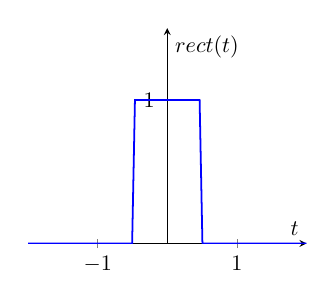
\begin{tikzpicture}[scale=0.8]
                        \begin{axis}[
                            domain=-2:2,
                            samples=100,
                            axis lines=middle,
                            xlabel={$t$},
                            ylabel={$rect(t)$},
                            ymin=0, ymax=1.5,
                            xmin=-2, xmax=2,
                            xtick={-1,0,1},
                            ytick={0,1},
                            height=5cm,
                            width=6cm
                        ]
                            \addplot[thick,blue] {abs(x) <= 0.5 ? 1 : 0};
                        \end{axis}
                    \end{tikzpicture}
                    \caption{$rect(t)$}
                \end{subfigure}
                \hfill
                % Sinc function
                \begin{subfigure}[b]{0.45\textwidth}
                    \centering
                    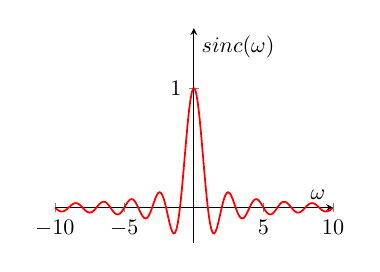
\begin{tikzpicture}[scale=0.8]
                        \begin{axis}[
                            domain=-10:10,
                            samples=200,
                            axis lines=middle,
                            xlabel={$\omega$},
                            ylabel={$sinc(\omega)$},
                            ymin=-0.3, ymax=1.5,
                            xmin=-10, xmax=10,
                            xtick={-10,-5,5,10},
                            ytick={1},
                            height=5cm,
                            width=6cm
                        ]
                            \addplot[thick,red] {x == 0 ? 1 : sin(deg(pi*x))/(pi*x)};
                        \end{axis}
                    \end{tikzpicture}
                    \caption{$\mathcal{F} \{rect(t)\}$ (Sinc function)}
                \end{subfigure}
            \end{figure}
        \end{block}
    }

    \only<35>{
        \begin{block}{Convolution}
            \begin{figure}
                \centering
                % Convolution of two rect functions
                \begin{subfigure}[b]{0.45\textwidth}
                    \centering
                    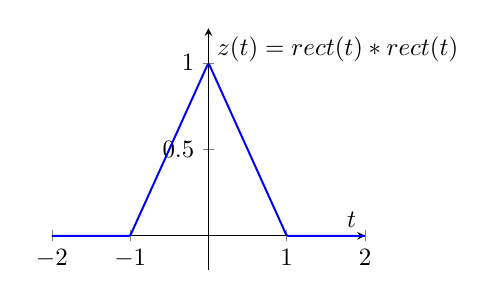
\begin{tikzpicture}[scale=0.9]
                        \begin{axis}[
                            domain=-2:2,
                            samples=200,
                            axis lines=middle,
                            xlabel={$t$},
                            ylabel={$z(t) = rect(t) * rect(t)$},
                            ymin=-0.2, ymax=1.2,
                            xmin=-2, xmax=2,
                            xtick={-2,-1,0,1,2},
                            ytick={0,0.5,1},
                            height=5cm,
                            width=6cm
                        ]
                            \addplot[thick,blue] {abs(x) <= 1 ? (1 - abs(x)) : 0};
                        \end{axis}
                    \end{tikzpicture}
                    \caption{$z(t) = rect(t) * rect(t)$}
                \end{subfigure}
                \hfill
                % Fourier Transform of convolution of two rect functions
                \begin{subfigure}[b]{0.45\textwidth}
                    \centering
                    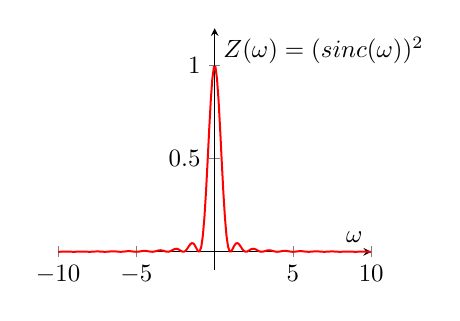
\begin{tikzpicture}[scale=0.9]
                        \begin{axis}[
                            domain=-10:10,
                            samples=200,
                            axis lines=middle,
                            xlabel={$\omega$},
                            ylabel={$Z(\omega) = (\text{sinc}(\omega))^2$},
                            ymin=-0.1, ymax=1.2,
                            xmin=-10, xmax=10,
                            xtick={-10,-5,0,5,10},
                            ytick={0,0.5,1},
                            height=5cm,
                            width=6cm
                        ]
                            \addplot[thick,red] {x == 0 ? 1 : (sin(deg(pi*x))/(pi*x))^2};
                        \end{axis}
                    \end{tikzpicture}
                    \caption{$Z(\omega) = \mathcal{F} \{z(t)\}$}
                \end{subfigure}
            \end{figure}
        \end{block}
    }
\end{frame}

\begin{frame}{Fourier Transform Properties (Table 1)}
    \begin{table}[ht]
    \centering
    \renewcommand{\arraystretch}{1.5}  % Adjust row height
    \small  % Reduce font size
        \begin{tabular}{|>{\columncolor{rowcolor1}}p{3cm}|>{\columncolor{rowcolor1}}p{3.5cm}|>{\columncolor{rowcolor1}}p{4.5cm}|}
            \hline
            \textbf{Property} & \textbf{Time Domain} & \textbf{Fourier Transform} \\
            \hline
            \rowcolor{rowcolor2}
            Linearity & \( x(t) = A x_1(t) + B x_2(t) \) & \( X(j\omega) = A X_1(j\omega) + B X_2(j\omega) \) \\
            \hline
            Time Shifting & \( x(t - t_0) \) & \( e^{-j\omega t_0} X(j\omega) \) \\
            \hline
            \rowcolor{rowcolor2}
            Conjugation & \( x^*(t) \) & \( X^*(-j\omega) \) \\
            \hline
            Differentiation in Time & \( \frac{d^n x(t)}{dt^n} \) & \( (j\omega)^n X(j\omega) \) \\
            \hline
            \rowcolor{rowcolor2}
            Differentiation in Frequency & \( -jt x(t) \) & \( \frac{dX(j\omega)}{d\omega} \) \\
            \hline
            Time Integration & \( \int_{-\infty}^t x(\tau)d\tau \) & \( \frac{1}{j\omega} X(j\omega) + \pi X(0)\delta(\omega) \) \\
            \hline
        \end{tabular}
    \end{table}
\end{frame}

\begin{frame}{Fourier Transform Properties (Table 2)}
    \begin{table}[ht]
    \centering
    \renewcommand{\arraystretch}{1.5}  % Adjust row height
    \small  % Reduce font size
        \begin{tabular}{|>{\columncolor{rowcolor1}}c|>{\columncolor{rowcolor1}}c|>{\columncolor{rowcolor1}}c|}
            \hline
            \textbf{Property} & \textbf{Time Domain} & \textbf{Fourier Transform} \\
            \hline
            \rowcolor{rowcolor2}
            Time Scaling & \( x(at) \) & \( \frac{1}{|a|} X\left(\frac{j\omega}{a}\right) \) \\
            \hline
            Time Reversal & \( x(-t) \) & \( X(-j\omega) \) \\
            \hline
            \rowcolor{rowcolor2}
            Frequency Shifting & \( x(t) e^{j\omega_0 t} \) & \( X(j(\omega - \omega_0)) \) \\
            \hline
            Duality & \( X(t) \) & \( 2\pi x(-j\omega) \) \\
            \hline
            \rowcolor{rowcolor2}
            Time Convolution & \( x(t) * h(t) \) & \( X(j\omega) H(j\omega) \) \\
            \hline
            Parseval's Theorem & \( \int_{-\infty}^\infty |x(t)|^2 dt \) & \( \frac{1}{2\pi} \int_{-\infty}^\infty |X(j\omega)|^2 d\omega \) \\
            \hline
            \rowcolor{rowcolor2}
            Modulation & \( z(t) = x(t) y(t) \) & \( Z(\omega) = \frac{1}{2\pi} X(j\omega) * Y(j\omega) \) \\
            \hline
        \end{tabular}
    \end{table}
\end{frame}

\begin{frame}{Fourier Transform Table}
    \begin{table}[ht]
    \centering
    \renewcommand{\arraystretch}{1.5}  % Adjust row height
        \begin{tabular}{|>{\columncolor{rowcolor1}}c|>{\columncolor{rowcolor1}}c|}
            \hline
            \textbf{Signal in Time Domain} & \textbf{Fourier Transform} \\
            \hline
            \rowcolor{rowcolor2}
            \( \delta(t) \) & \( 1 \) \\
            \hline
            \( u(t) \) & \( \frac{1}{j\omega} + \pi \delta(\omega) \) \\
            \hline
            \rowcolor{rowcolor2}
            \( \delta(t - t_0) \) & \( e^{-j\omega t_0} \) \\
            \hline
            \( t e^{-a t} u(t) \) & \( \frac{1}{(a + j\omega)^2} \) \\
            \hline
            \rowcolor{rowcolor2}
            \( u(-t) \) & \( \pi \delta(\omega) - \frac{1}{j\omega} \) \\
            \hline
            \( e^{at} u(-t) \) & \( \frac{1}{a - j\omega} \) \\
            \hline
        \end{tabular}
    \end{table}
\end{frame}

\begin{frame}{Fourier Transform Table}
    \begin{table}[ht]
    \centering
    \renewcommand{\arraystretch}{1.5}  % Adjust row height
        \begin{tabular}{|>{\columncolor{rowcolor1}}c|>{\columncolor{rowcolor1}}c|}
            \hline
            \textbf{Signal in Time Domain} & \textbf{Fourier Transform} \\
            \hline
            \rowcolor{rowcolor2}
            \( e^{-a|t|} \) & \( \frac{2a}{a^2 + \omega^2} \) \\
            \hline
            \( \cos(\omega_0 t) \) & \( \pi [\delta(\omega - \omega_0) + \delta(\omega + \omega_0)] \) \\
            \hline
            \rowcolor{rowcolor2}
            \( \sin(\omega_0 t) \) & \( -j \pi [\delta(\omega - \omega_0) - \delta(\omega + \omega_0)] \) \\
            \hline
            \( \frac{1}{a^2 + t^2} \) & \( e^{-a|\omega|} \) \\
            \hline
            \rowcolor{rowcolor2}
            \( \text{Sgn}(t) \) & \( \frac{2}{j\omega} \) \\
            \hline
            \( 1 \, \text{(for all t)} \) & \( 2\pi \delta(\omega) \) \\
            \hline
        \end{tabular}
    \end{table}
\end{frame}

\end{document}
